\documentclass[times, 10pt, twocolumn]{article}
\usepackage{amsmath,amsfonts,amsthm,amssymb}
\usepackage{fancyhdr}
\usepackage{chngpage}
\usepackage{color}
\usepackage{graphicx}
\usepackage{boxedminipage}
\usepackage{enumerate}
\usepackage{latex8}
\usepackage{times}
\usepackage[utf8]{inputenc}


\title{DADSTORM\\A simple, fault-tolerant and real-time stream processing system}
\author{DAD 2016-2017\\ Group 12:
\\ Daniel Fermoselle nº 78207
\\ João Marçal nº 78471
\\ Tiago Rodrigues nº 78692
}
\begin{document}
\maketitle
\date

\begin{abstract}
DADSTORM is a simple but reliable stream processing system. It's mainly used by Instituto Superior Tecnico Students.
\\The main features are: the 3 possible semantics of tuple processing it can have, fault-tolerance to f faults per operator with a synchronous model of detection, 3 modes of tuple routing and last but the not the least 
5 types of operators.
This system is composed by a Puppet Master, Process Creation Service, Operators with their Replicas, Tuples and ThreadPools.
\end{abstract}

%------------------------------------
\section{Introduction}
Nowadays with the rising interest on big data, streaming information is getting more and more important and we want to process that data as fast as possible even though the possibility of having faults still exists.
In order to get that information in a reliable way we developed DADSTORM. This system is reliable through the passive replication we use, allowing us to get tolerance to f faults using just f+1 replicas. 
\\Our system process tuples based on the type of operator which can be UNIQ, COUNT, DUP, FILTER and CUSTOM. With these operators we can get the data processed in a way that let us get the information we want.

%------------------------------------
\section{Programming Model}
In this section, we provide a high-level overview of the programming model, highlighting the key concepts. 
\\In DADSTORM data is represented as string Tuples, i.e, a collection of strings.
\\To begin with we have a puppet master who will start all the operators on all the machines with the help of the process creation service the later will already be located in all the machines that will run operator replicas.
\\The puppet master has an intuitive interface inside which we have a box where we can introduce a path to a configuration file (see figure 1) to start all the operator's replicas as well as their inputs, routing, operator spec and address.
\begin{figure}
  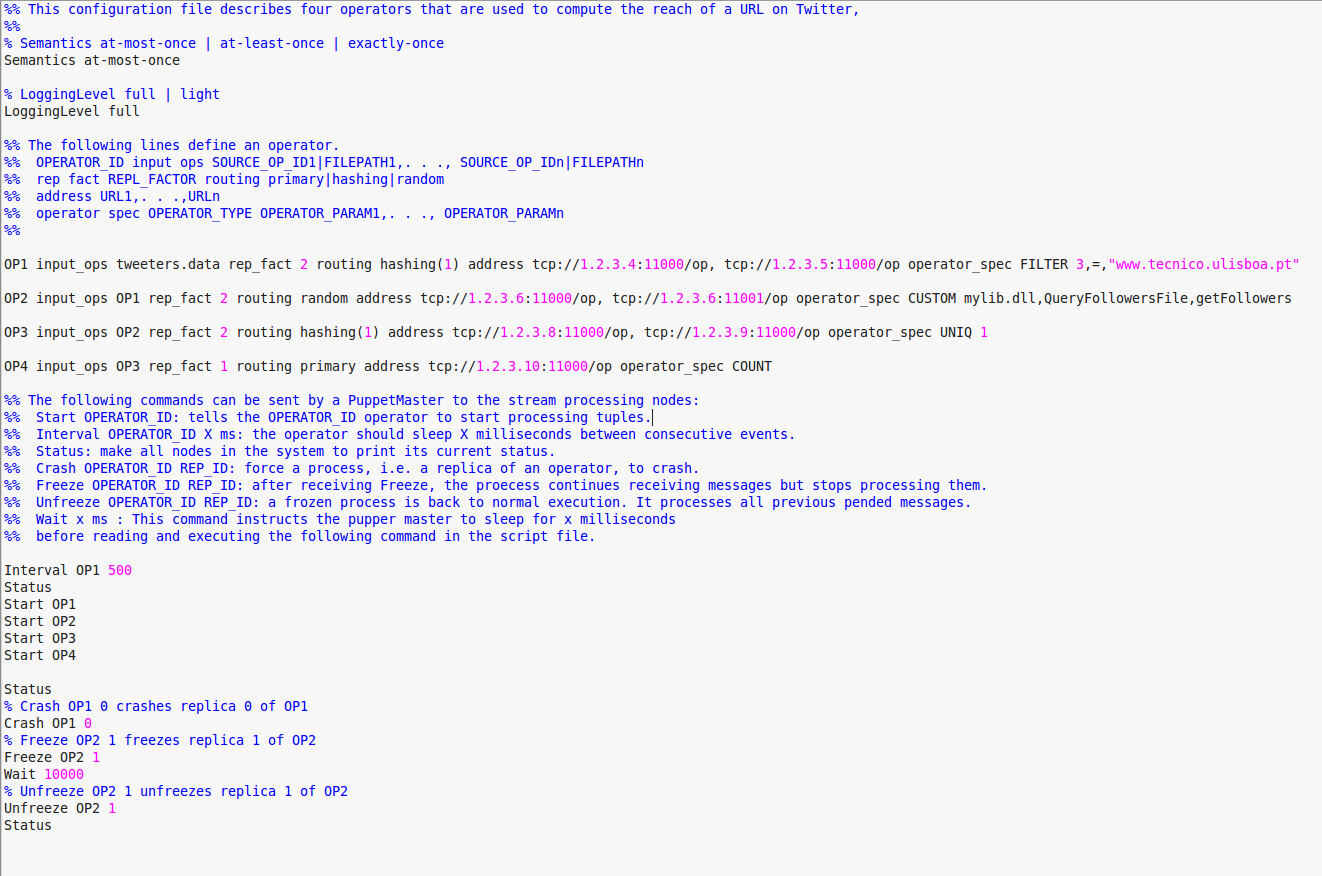
\includegraphics[width=\linewidth]{configFileExample.PNG}
  \caption{An example of a config file.}
\end{figure}
\\The tuples are stored inside a file that will be accessed by the first operator of the stream. The operators are composed by replicas which can be located inside different machines.
\\All the replicas might fail but we assure f fault tolerance to silent failures for each operator. We assume that none of the first operator replicas can fail and that there is at least one replica alive per operator, in order to guarantee that, we have to have at least f+1 replicas for each operator, being f the number of fautls of each operator.
\\A quick overall. So first of all we start the puppet master which will through, the configuration file introduced and with the help of the process creation service, create all the operator's replicas. Then the replicas of the first operator will read the .dat file which has the begining tuples to be processed. After this initialization all the replicas will receive tuples and process them, sending the result to the next operators, unless it is a replica of the last operator this one doesn't send anything, it just processes tuples.
\\To finish this section the user of our system doesn't have to worry about how the system is distributing the operations, the user just has to create the configuration file and let the puppet master read it, then just execute and all the data will be processed, getting in the end the desired information.



%------------------------------------
\section{DADSTORM Abstractions}
In this section we will talk a little bit about the abstractions we created for this system, begining with the tuple and all its variations, having an overview about the operator, the replicas. To finish the section we will talk about the parser, the RepInfo and the ConfigInfo.



%------------------------------------
\subsection{Tuple}
Tuple, this is one of the most important abstractions of our system if not the most one. The Tuple is a possible infinite collection of strings, it also has a unique id to be used when the tuple processing semantics requires so. The tuples are processed and when this happens it is created another tuple having as content the result of processing the previous tuple. 
\\To help mostly the processing semantics we created also 3 more variations of the tuple, which are: AckTuple, TimerTuple and Tuple2TupleProcessed. 
\\The AckTuple is no more than a tuple associated with the url of the replica who sent the tuple this url can be used in the future. 
\\The TimerTuple is a tuple associated with a timer of the limit the tuple has to be acked, otherwise it'll be resent. 
\\Last but not the least there is the Tuple2TupleProcessed this abstraction contains 2 tuples, the first tuple when processed by some replica generates the second tuple, this association can be useful first to compare if the tuple was already processed and then to return the result of processing the first tuple if necessary.


%------------------------------------
\subsection{RepInfo}
RepInfo is an abstraction that basically gives all the information that a replica of an operator has to know. It has the notion of replica routing, its parameters as well as the urls of the replicas to which will be sent tuples, the url of the replica, the operator spec i.e what operation the replica will perform, the id of the replica, the sibling replicas i.e the replicas from the same operator. 
\\In short the RepInfo has all the information that a replica needs to know.
\\The RepInfo has a lot of information for one replica(this replica), more specifically: \textbf{routing}, the type of routing for this replica, \textbf{routingParam}, the parameters of the tuple to which the routing will be applied in this replica, \textbf{nextRouting}, the type of routing for the possible next replicas, \textbf{nextRoutingParam},the parameters of the tuple to in which the routing will be applied in the possible next replicas, \textbf{operatorSpec}, the type of this replica operator, \textbf{operatorParam}, the parameters of the tuple on which this replica operatorSpec will be applied, \textbf{sendInfoUrls}, the urls of the next replicas, \textbf{port}, this replica port, \textbf{loggingLvl},the type of logging that the system is configured for, \textbf{input}, the input operators or file of this replica, this is mainly used to get the file.dat, \textbf{pmsUrl}, the url of the puppet master, \textbf{siblingsUrls},the urls of the other replicas of the same operator, \textbf{myUrl}, the url of this replica, \textbf{semantics}, the semantics the system in running, \textbf{receiveInfoUrls}, the urls of the replicas which can send tuples to this replica, \textbf{operatorId} the id of this replica's operator. With all this information the system can know which replicas should have the copy of the state in case of failure (siblings), which replicas will receive the tuples processed (sendInfoUrls), the type of operator (operator spec).


%------------------------------------
\subsection{Operators and Replicas}
In this section we will talk mostly about replicas because they are simply what an operator is.
\\A replica basically is an object that reads tuples from possibly infinite inputs, processes and finally sends them to the next replicas in the chain.
\\Each replica has a thread pool which will have 2 threads one for reading tuples and processing them and another thread to send the processed tuples to the next replicas. Each thread has a circular buffer in which the tuples will be waiting to be read and processed or sent. The replicas also have a RepInfo that is defined above, this structure is very important for the replica.
\\Replicas have a few fundamental functions: Start, processTuple, SendTuple.
\\\textbf{Start(RepInfo info)}: Start is the function that allows the replica to start it gets as argument a RepInfo that will be the replica RepInfo. This function starts all the failure detection timers as well as the most important lists, also if the replica is one of the first operators replica it will read tuples from the .dat file and process them.
\\\textbf{processTuple(Tuple t)}: This function receives a tuple t as argument and will process it with the operator spec of the replica, adding the tuple t or the result of processing to a list of acks or replication if necessary. In the end of processing it the result will be put in the circular buffer of the processed tuples in order to be then send.
\\\textbf{SendTuple(Tuple t, bool resend}: This function receives a tuple t and a boolean resend, the tuple is the tuple that will be send accordingly to the sending policy of the next operator's replicas, the boolean resend indicates if this tuple is being send for the first time or not if it is some lists of tuples that need to be ack will not be updated.



%------------------------------------
\subsection{Parser}
The parser is an abstraction used by the puppet master in order to process the configuration file, this parser receives the path to the configuration file and gives to the puppet master an array of ConfigInfo with all the information of the operators and its replicas as well as the list of commands that the puppet master will have to execute.





%------------------------------------
\subsection{ConfigInfo}
This abstraction is almost the same as the RepInfo but for the puppet master. It's through the ConfigInfo that the puppet master can know how to start the replicas with which properties that in the correct time will be sent to the replicas inside the RepInfo



%------------------------------------
\section{Architecture and Implementation}
In this section we will describe in more detail what each component of the architecture of our solution does and how it was implemented.




%------------------------------------
\subsection{Tuple}
As said in section 3.1 the tuple is the base of our whole system. The tuple contains a collection of strings and an unique id, this id is composed by the operator name concatenated with the replica index plus an unique id inside that replica. This first basic tuple is sent between replicas and gets changed every time it's processed. The AckTuple is the first sub-type of tuples and each operator saves an array list with this object until the tuple is acked, this sub-type plus the TimerAck which has the timer to receive ack before resend the tuple work together to guarantee that the tuple is at least received once. Now the last sub-type of tuple is Tuple2TupleProcessed this tuple saves the pair \textless Tuple, TupleProcessed\textgreater and it's used as a method to let the replica know if the tuple was already processed comparing the id's of the tuple receive and all the pairs Tuple2TupleProcessed saved in an array in each replica.



%------------------------------------
\subsection{Operators and Replicas}
The notion of operator is as said before a little bit abstracted as a collection of replicas, that being said in this subsection we will only talk about replicas. 
\\The key of the replicas is to mantain state as well as tracking all the tuples, with use arrays and list to do this.
\\Replicas are implemented as object which have a few structures inside: one threadpool, one RepInfo, one status and a few array lists that will be explained in the end of this sub-section.
\\First of all the threadpool, this atribute mantains a reference to access the replica threadpool that has 2 threads: one to read and process and another to send tuples. Each of this threads has a circular buffer where the tuples are stored while waiting to be consumed. When the circular buffer gets full it will block the reception until there is a consume action. One of the threads will be constantly running a ConsumeRead method that consumes tuples from the circular buffer, reads it and with the replica operator spec processes it, after that, the tuple is sent to the circular buffer of the thread which is always running a ConsumeProcessed method, this thread will take a tuple from its circular buffer and with the replica is going to send to the right next replica.
\\The status of a replica indicates if it's working or not and there is also information about the replica being frozen.
\\A very important part of the replicas is how do they react to the different semantics. We have 3 semantics: at most once, at least once and exactly once.
\\\textbf{At most once}: This semantic doesn't need any other kind of structures or treatment to deal with because if the tuple was not sent or processed there is no problem.
\\\textbf{At least once}: When dealing with this semantic it gets trickier because we need to guarantee the tuple is at least processed one time. So to solve this issue everytime we send a tuple in the sender replica we add the tuple to a list(ToReceiveAck), this list tracks all the tuples that need to receive an ack, also, we add the tuple to a list(TimerAck) associated with a timer which is programmed to after 10 seconds resend the tuple if an ack for that tuple wasn't received yet, when the sender replica receives the ack for that tuple the timer is disposed and the tuple removed from the ToReceiveAck list.
\\Now about the receiver, when the sender, sends the replica it also adds to a list (ToBeAcked) in the receiving replica the tuple sent plus the url which sent the tuple, when this replica processes the tuple it sends an ack to one replica of the previous operator, this ack will then be propagated inside the operator to reach every replica and ack the tuple on all of them, also after processing the tuple the receiving replica will remove the tuple from the ToBeAcked list, as the tuple was already acked.
\\\textbf{Exactly once}: Regarding now with this semantics all of what was said to at least once is applied to this semantics but with more. In this semantic everytime a tuple is being processed it is checked if it was already processed, if not then the tuple and the result of processing it is combined(Tuple2TupleProcessed) and added to a list(TupleToTupleProcessed) and propagated to the replica siblings, if the tuple was already processed then the tuple is rejected and not processed again.
\\\textbf{Fault tolerance}: To assure fault tolerance some replication methods had to be applied, so we do it this way. First every time a replica processes a tuple that tuple is added to a list(ReplicatedTuples) in each of the replica siblings, this list as the name states saves all the tuples that are being processed by a replica.
\\Now what happens when a replica fails. If the replica is idle and all the tuples it processed are acked as well as the all the tuples it sent already received ack then nothing happens and a sibling replica will take the place of the failed one when needed. If the replica fails before sending an ack to the previous replica there is no problem because when the sibling replica takes the place it will receive a resent tuple and ack it then. Finally if a replica is waiting for an ack and dies there is no problem because the receiving replica will send the ack to at least one of the replicas of the previous operator which sent it the tuple. But what happens if the replica still has tuples to send, then thanks to the ReplicatedTuples list each of the replica siblings will process the not already processed tuples accordingly to the routing of the operator with the still alive replicas.




%------------------------------------
\subsection{Puppet Master}
The puppet master provides an interface between the system, the replicas and the user.
The puppet master 
//TODO WHAT TO SAY




%------------------------------------
\subsection{Process Creation Service}
The process creation service was created just to allow the puppet master to contact him through the shared common class which allow the puppet master to create the replicas of the operators in the machines where the process creation service is running.



%------------------------------------
\subsection{Failure Recovery}
Our system as already said has f+1 replicas per operator in order to guarantee faul-tolerance to f silent failures. This is guaranteed in a synchronous model because each replica has two timers, one that every 12 seconds sends a ping to the replica siblings, i.e the replicas that are part of the same operator, and another that every 12 seconds sends a ping to the replica children, i.e the replicas that receive tuples from this one.
\\If the first timer ping doesn't get response from one sibling that sibling is removed from the list and all the tuples that were being saved in shared array of replicated tuples are reprocessed by the replica that should after the death of the other reprocess the tuples and sent to the right receiving operator's replica.
\\Now about the second timer, if a child doesn't ping back it's simply removed from the possible sendInfoUrl, i.e the possible urls of replicas that can receive tuples from this one, in order to forbid the sender to wrongly send tuples to a dead replica.



%------------------------------------
\section{Production Experiences}
This section highlights our experiences with developing DADSTORM the difficulties we encountered and what we think about our implementation.
\\So in the first part of the project until the checkpoint we didn't have that much difficulty doing it but we only started implementing the operators in the week of the delivery of the checkpoint and as we had more project to do this checkpoint got a bit delayed.
\\The first difficulty that we realy encountered was when we started implementing the semantics mostly the at least once because we didn't have an idea on how to do it but we had a discussion between all the members and we tested a few concepts like tuples that knew what url they had to send ack, but then we thought (what would happen if the replica with that url was already dead?).
\\Then we also had difficulty with the failure recovery because at first we didn't thought about the timers and we started thinking about active replication but then we reached the conclusion that passive replication synchronously with the timers was easier for us and with a better performance than active replication, but we think that we could have improved it even better. 




%------------------------------------
\section{Evaluation}
All the following tests were done in localhost.
Since we finished the project we tested a few cases. First we tested a normal run, without failures neither freezes, using at most once semantics which took 7 seconds to finish with correct result, the at least once took 13 seconds to finish with correct result and the exactly once last for 12 seconds to finish with correct result. Then we tested with failures and freezes and we get these values, using at most once it took 10 seconds and didn't process some tuples, using at least once lasted for 1 minute and 13 seconds to finish with some tuples being sent more than once, exactly once took 50 seconds to finish but processed exactly once each tuple that needed to.
\\With the above evaluation we reached the conclusion that as expected with failures all semantics take longer and that the exactly once semantic grants us a good compromise between time and assurance.





%------------------------------------
\section{Conclusion}
In conclusion our DADSTORM implementation is good, we think we reached all the objectives, our system supports f failures, different semantics and gets the desired information although it could be faster.
\\It could be even better with more time, but that is always the same thing everyone says.


\end{document}
